\documentclass[12pt]{article}
\usepackage[left=1cm, right=1cm, top=2cm,bottom=1.5cm]{geometry} 

\usepackage[parfill]{parskip}
\usepackage[utf8]{inputenc}
\usepackage[T2A]{fontenc}
\usepackage[russian]{babel}
\usepackage{enumitem}
\usepackage[normalem]{ulem}
\usepackage{amsfonts, amsmath, amsthm, amssymb, mathtools}
\usepackage{tikz}
\usepackage{tabularx}
\usepackage{hhline}

\usepackage{accents}
\usepackage{fancyhdr}
\pagestyle{fancy}
\renewcommand{\headrulewidth}{1.5pt}
\renewcommand{\footrulewidth}{1pt}

\usepackage{graphicx}
\usepackage[figurename=Рис.]{caption}
\usepackage{subcaption}
\usepackage{float}

%%Наименование папки откуда забирать изображения
\graphicspath{ {./images/} }

%%Изменение формата для ввода доказательства
\renewcommand{\proofname}{$\square$  \nopunct}
\renewcommand\qedsymbol{$\blacksquare$}

%%Изменение отступа на таблицах
\addto\captionsrussian{%
	\renewcommand{\proofname}{$\square$ \nopunct}%
}
%% Римские цифры
\newcommand{\RN}[1]{%
	\textup{\uppercase\expandafter{\romannumeral#1}}%
}

%% Для удобства записи
\newcommand{\MR}{\mathbb{R}}
\newcommand{\MQ}{\mathbb{Q}}
\newcommand{\MC}{\mathbb{C}}
\newcommand{\MI}{\mathrm{I}}
\newcommand{\MJ}{\mathrm{J}}
\newcommand{\MH}{\mathrm{H}}
\newcommand{\MT}{\mathrm{T}}
\newcommand{\MU}{\mathcal{U}}
\newcommand{\MV}{\mathcal{V}}
\newcommand{\VN}{\varnothing}
\newcommand{\VE}{\varepsilon}
\newcommand{\id}{\mathrm{id}}

\theoremstyle{definition}
\newtheorem{defn}{Опр:}
\newtheorem{rem}{Rm:}
\newtheorem{prop}{Утв.}
\newtheorem{exrc}{Упр.}
\newtheorem{lemma}{Лемма}
\newtheorem{theorem}{Теорема}
\newtheorem{corollary}{Следствие}

\newenvironment{cusdefn}[1]
{\renewcommand\thedefn{#1}\defn}
{\enddefn}

\DeclareRobustCommand{\divby}{%
	\mathrel{\text{\vbox{\baselineskip.65ex\lineskiplimit0pt\hbox{.}\hbox{.}\hbox{.}}}}%
}
%Короткий минус
\DeclareMathSymbol{\SMN}{\mathbin}{AMSa}{"39}
%Длинная шапка
\newcommand{\overbar}[1]{\mkern 1.5mu\overline{\mkern-1.5mu#1\mkern-1.5mu}\mkern 1.5mu}
%Функция знака
\DeclareMathOperator{\sgn}{sgn}

%Обозначение константы
\DeclareMathOperator{\const}{\text{const}}

%Интеграл в большом формате
\DeclareMathOperator{\dint}{\displaystyle\int}

\newcommand{\smallerrel}[1]{\mathrel{\mathpalette\smallerrelaux{#1}}}
\newcommand{\smallerrelaux}[2]{\raisebox{.1ex}{\scalebox{.75}{$#1#2$}}}

\newcommand{\smallin}{\smallerrel{\in}}
\newcommand{\smallnotin}{\smallerrel{\notin}}

\newcommand*{\medcap}{\mathbin{\scalebox{1.25}{\ensuremath{\cap}}}}%
\newcommand*{\medcup}{\mathbin{\scalebox{1.25}{\ensuremath{\cup}}}}%

%Скалярное произведение
\DeclarePairedDelimiterX{\inner}[2]{\langle}{\rangle}{#1, #2}

%Подпись символов снизу
\newcommand{\ubar}[1]{\underaccent{\bar}{#1}}

\newcommand*\circled[1]{\tikz[baseline=(char.base)]{
		\node[shape=circle,draw,inner sep=2pt] (char) {#1};}}


\begin{document}
\lhead{Линейная алгебра}
\chead{Мануйлов В.М.}
\rhead{Лекция - 4}
\section*{Двойственное пространство и линейные функции}
Пусть $V$ - линейное пространство, $l \colon V \to \mathbb{K}$ - линейные функции $\Rightarrow V^\prime$ - двойственное пространство. $\dim{V} = \dim{V^\prime}\colon e_1,\dotsc, e_n$ - базис $V \Rightarrow \VE^1, \dotsc, \VE^n$ - двойственный базис в $V^\prime, \, l_i = l(e_i)$.

\begin{lemma}
	$l_i$ - координаты линейной функции $l$ в базисе $\VE^1,\dotsc, \VE^n$.
\end{lemma}
\begin{proof}
	Линейные функции: $l_1 \VE^1 + \dotsc + l_n \VE^n, \, f = g \Leftrightarrow f(x) = g(x), \, \forall x$.
	
	Пусть $x \in V \Rightarrow$ подставим в $l$ и в линейную функцию: 
	$$
		x = x^1 e_1 + \dotsc + x^n e_n \Rightarrow (l_1 \VE^1 + \dotsc + l_n \VE^n)(x) = (l_1 \VE^1 + \dotsc + l_n \VE^n)(x^1 e_1 + \dotsc + x^n e_n) = 
	$$
	$$	
		= l_1 \VE^1(x^1 e_1 + \dotsc + x^n e_n) + \dotsc + l_n \VE^n(x^1 e_1 + \dotsc + x^n e_n) = x^1 l_1 + \dotsc + x^n l_n
	$$
	Знаем, что  $\VE^i(e_j) = \delta_j^i = \begin{cases} 1, & i = j\\ 0, & i \neq j \end{cases}$ - символ Кронекера. 
	$$
		l(x) = l(x^1 e_1 + \dotsc + x^n e_n) = x^1 l(e_1) + \dotsc + x^n l(e_n) = x^1 l_1 + \dotsc + x^n l_n \Rightarrow
	$$ 
	$\Rightarrow$ функции совпадают $\Rightarrow l = l_1 \VE^1 + \dotsc + l_n \VE^n \Rightarrow l_1, \dotsc, l_n$ - координаты $l$ в базисах $\VE^1, \dotsc, \VE^n$.
\end{proof}

\uline{Сокращенная форма записи}: $l(x) = x^i l_i$.

Пусть $e_1,\dotsc, e_n$ и $\tilde{e}_1, \dotsc, \tilde{e}_n$ - базисы в $V$, $\tilde{e}_i = c_i^j e_j$, $c_i^j$- элементы матрицы перехода. $\VE^1,\dotsc,\VE^n$ - двойственный к $(e)$ базис, $\tilde{\VE}^1,\dotsc, \tilde{\VE}^n$ - двойственный к $(\tilde{e})$ базис.

В базисе $(\VE)$ функция $l$ имеет координаты $l_1,\dotsc, l_n$. 

В базисе $(\tilde{\VE})$ функция $l$ имеет координаты $\tilde{l}_1,\dotsc, \tilde{l}_n$.
$$
	 \tilde{l}_i = l(\tilde{e}_i) = l(c_i^j e_j) = c_i^j l_j = c_i^1 l_1 + \dotsc + c_i^n l_n
$$
\begin{lemma}
	Координаты линейной функции при переходе от одного базиса к другом меняются по формуле $\tilde{l}_i = c_i^jl_j$.
\end{lemma}
\begin{rem}
	$x^i = c_j^i \tilde{x}^j$.
\end{rem}
\textbf{Пример}: Двойственно пространство к $\mathbb{K}_n[t]$. Пусть $p(t)$ - многочлен, $p(t_0)$ - число. Можно утверждать следующее:
\begin{itemize}
	\item подставить $\rightarrow$ сложить два многочлена $\Leftrightarrow$ сложить два многочлена $\rightarrow$ подставить;
	\item подставить $\rightarrow$ умножить  $\Leftrightarrow$ умножить $\rightarrow$ подставить;
\end{itemize}
Таким образом, функция, сопоставляющая многочленам их значения в $t_0$ - линейная:
$$ev_{t_0}(p) = p(t_0)$$

\begin{lemma}
	Пусть $t_0, t_1, \dotsc, t_n$ - попарно различны, тогда $ev_{t_0}, ev_{t_1}, \dotsc, ev_{t_n}$ - образуют базис в двойственном пространстве $(\mathbb{K}_n[t])^\prime$.
\end{lemma}
\begin{proof}
	Найдем в $\mathbb{K}_n[t]$ базис для которого этот базис ($ev_{t_0}, ev_{t_1}, \dotsc, ev_{t_n}$) будет двойственным:
	$$
		p_0, p_1, \dotsc, p_n \in \mathbb{K}_n[t]\colon ev_{t_0}(p_i) = \begin{cases} 1,& i = 0\\ 0, & i \neq 0 \end{cases}, \dotsc, ev_{t_n}(p_i) = \begin{cases} 1,& i = n\\ 0, & i \neq n \end{cases} \Leftrightarrow p_j(t_i) = \begin{cases} 1, & i = j\\ 0, &  i \neq j \end{cases}
	$$
	Построим многочлен $(t - t_1){\cdot} \dotsc {\cdot}(t - t_n) \Rightarrow (t_0 - t_1){\cdot}\dotsc{\cdot}(t_0 - t_n) \neq 0 \Rightarrow$ 
	$$
		p_0(t) = \dfrac{(t-t_1){\cdot}\dotsc{\cdot}(t-t_n)}{(t_0 - t_1){\cdot}\dotsc{\cdot}(t_0 - t_n)}, \dotsc, p_n(t) = \dfrac{(t-t_0){\cdot}\dotsc{\cdot}(t-t_{n-1})}{(t_n - t_0){\cdot}\dotsc{\cdot}(t_n - t_{n-1})}, \, p_i(t) = \dfrac{\prod\limits_{j \neq i}(t-t_j)}{\prod\limits_{j \neq i}(t_i-t_j)} \Rightarrow p_j(t_i) = \begin{cases} 1,& i = j\\ 0, & i \neq j \end{cases}
	$$
	Возьмем линейную комбинацию $\lambda_0 ev_{t_0} + \dotsc + \lambda_n ev_{t_n} = 0$ (равенство двух линейных функций: лин. комбинации и нуля), подставим $p_i \Rightarrow \lambda_0 ev_{t_0}(p_i) + \dotsc + \lambda_n ev_{t_n}(p_n) = \lambda_i ev_{t_i}(p_i) = \lambda_i = 0, \, \forall i = \overline{1,n} \Rightarrow$ линейно независимы.
	Так как $\dim{\mathbb{K}_n[t]} = n+1 = \dim{(\mathbb{K}_n[t])^\prime} \Rightarrow$ линейная независимость и максимальный набор $\Rightarrow$ базис.
\end{proof}
\begin{exrc}
	Доказать, что $p_0, p_1, \dotsc, p_n$ - базис в $\mathbb{K}_n[t]$.
\end{exrc}
\section*{Линейные функции на $V^\prime$}

Пусть $x \in V, \, l \in V^\prime, \, \varphi_x(l) \coloneqq l(x), \, \varphi_x \colon V^\prime \to \mathbb{K}$. Будут выполнены следующие выражения:
\begin{enumerate}[label ={(\arabic*)}]
	\item Пусть $l, \, l^\prime \in V^\prime$, тогда $\varphi_x(l+ l^\prime) = (l + l^\prime)(x) = l(x) + l^\prime(x) = \varphi_x(l) + \varphi_x(l^\prime)$;
	\item Пусть $l \in V^\prime, \, \lambda \in \mathbb{K}$, тогда $\varphi_x(\lambda {\cdot} l) = (\lambda  {\cdot} l)(x) = \lambda {\cdot} l(x) = \lambda {\cdot} \varphi_x(l)$;
\end{enumerate}
Таким образом, каждый $x \in V$ задает линейную функцию на $V^\prime$. 

$V \rightarrow V^\prime \rightarrow (V^\prime)^\prime, \, \varphi_x(l) \in (V^\prime)^\prime$ - второе двойственное пространство. $\dim{(V^\prime)^\prime} = \dim{V^\prime} = \dim{V}$. $\forall x \in V$ сопоставляем $\varphi_x \in (V^\prime)^\prime \Rightarrow$ получаем отображение:
$$F \colon x \mapsto \varphi_x, \, F\colon V \rightarrow (V^\prime)^\prime$$

\begin{lemma}
	$F$ является изоморфизмом $V \simeq (V^\prime)^\prime$.
\end{lemma}
\begin{proof}\hfill\\
	\uline{\textbf{Линейность}}: $\forall x, \, x^\prime \in V,\, F(x+x^\prime) = \varphi_{x + x^\prime},\, F(x) + F(x^\prime) = \varphi_x + \varphi_{x^\prime}$, так как это функции $\Rightarrow$ нужно подставлять аргументы:
	\begin{enumerate}[label ={\arabic*)}]
		\item $\varphi_{x+x^\prime}(l) = l(x + x^\prime) = l(x) + l(x^\prime), \, (\varphi_x + \varphi_{x^\prime})(l) = \varphi_x(l) + \varphi_{x^\prime}(l) = l(x) + l(x^\prime) = \varphi_{x+x^\prime}(l) \Rightarrow$ совпадают;
		\item $\forall x \in V,\, \forall \lambda \in \mathbb{K},\, F(\lambda x) = \varphi_{\lambda x}, \, \lambda F(x) = \lambda \varphi_x \Rightarrow \varphi_{\lambda x}(l) = l(\lambda x) = \lambda l(x),\, \lambda \varphi_x(l) = \lambda l(x) \Rightarrow$ совпадают;
	\end{enumerate}
	Таким образом, $F$ - линейное отображение.
	
	\uline{\textbf{Инъективность}}: $x,y \in V, \, F(x) = \varphi_x = \varphi_y = F(y)$, функции равны $\Leftrightarrow$ они равны на каждом аргументе, то есть 
	$$
		\varphi_x(l) = \varphi_y(l),\, \forall l \in V^\prime \Leftrightarrow l(x) = l(y), \, \forall l \in V^\prime \Leftrightarrow l(x - y) = 0, \, \forall l \in V^\prime
	$$ 
	Если $x - y \neq 0$ возьмем базис $e_1 = x - y \neq 0, e_2,\dotsc,e_n$, пусть $l = \VE^1$, поскольку утверждение выше верно для любой линейной функции  $(\forall l \in V^\prime) \Rightarrow \VE^1(e_1) = 1 \Rightarrow$ противоречие $\Rightarrow x = y$.
	
	\uline{\textbf{Сюръективность}}: Пусть $e_1, \dotsc, e_n$ - базис в $V$, рассмотрим $\varphi_{e_1}, \dotsc, \varphi_{e_n}$ - проверим их линейную независимость $\lambda_1 \varphi_{e_1} + \dotsc + \lambda_n \varphi_{e_n} = 0$ - на каждом аргументе. Подставим $\VE^i \Rightarrow \lambda_1 \varphi_{e_1}(\VE^i) + \dotsc + \lambda_n \varphi_{e_n}(\VE^i) = 0 \Rightarrow$
	$$
		\lambda_1 \VE^i(e_1) + \dotsc + \lambda_i \VE^i(e_i) + \dotsc + \lambda_n \VE^i(e_n) = \lambda_i = 0, \, \forall i = \overline{1,n}
	$$
	Таким образом, эти линейные функции линейно независимы. Так как, $\dim{(V^\prime)^\prime} = \dim{V} = n \Rightarrow \varphi_{e_1}, \dotsc, \varphi_{e_n}$, образуют базис $(V^\prime)^\prime$. Тогда 
	$$
		\forall \varphi \in (V^\prime)^\prime, \, \varphi = \lambda_1 \varphi_{e_1} + \dotsc + \lambda_n \varphi_{e_n} = \varphi_{\lambda_1 e_1 + \dotsc + \lambda_n e_n} \Rightarrow
		\varphi = F(\underbrace{\lambda_1 e_1 + \dotsc + \lambda_n e_n}_{\in V})
	$$ 
	то есть, линейные функции - сюръективны $\Rightarrow$ получим биекцию $\Rightarrow F$ является изоморфизмом.
\end{proof}

\begin{defn}
	Если данный изоморфизм не зависит от выбора системы координат - инвариантным спосбом, то такие изоморфизмы будем называть \uwave{каноническими}.
\end{defn}
\begin{defn}
	Отображение $F$ определено \uwave{инвариантно} относительно системы координат $\Rightarrow$ от неё не зависит.
\end{defn}

\section*{Сумма и пересечение подпространств}

$L_1, L_2$ - линейные подпространства в $V$, $L_1 \cap L_2$ - линейное подпространство в $V$. Проверим это:
\begin{enumerate}[label ={(\arabic*)}]
	\item $a,b \in L_1 \cap L_2 \Rightarrow a,b \in L_1, \, a, b \in L_2 \Rightarrow a + b \in L_1, \, a + b \in L_2 \Rightarrow a + b \in L_1 \cap L_2$;
	\item $a \in L_1 \cap L_2 \Rightarrow a \in L_1, \, a \in L_2 \Rightarrow \lambda a \in L_1, \, \lambda a \in L_2, \, \lambda \in \mathbb{K} \Rightarrow \lambda a \in L_1 \cap L_2$;
\end{enumerate}
таким образом, $L_1 \cap L_2$ - линейное подпространство в $V$.

$L_1 \cup L_2$ - линейное подпространство $\Leftrightarrow L_1 \subset L2 \vee L_2 \subset L_1$, иначе $L_1 \cup L_2$ - не линейное подпространство в общем случае.

\textbf{Пример}: $a \in L_1, \, b \in L_2, \, a + b \notin L_1 \cup L_2$.
\begin{figure}[H]
	\centering
	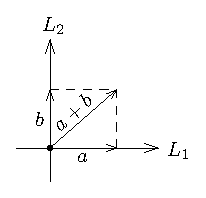
\includegraphics[width=0.18\textwidth]{4_1.eps}
	\caption{$L_1 \cup L_2$ не является линейным подпространством.}
	\label{4_1}
\end{figure}

\begin{defn}
	\uwave{Суммой линейных подпространств} $L_1 + L_2 = \langle L_1, L_2 \rangle = \{\, a + b \colon a \in L_1, \, b \in L_2 \,\}$.
\end{defn}

\begin{lemma}
	$L_1 + L_2$ является линейным подпространством.
\end{lemma}
\begin{proof}
	Пусть $a,b \in L_1 + L_2 \Rightarrow \exists \, a_1 \in L_1, a_2 \in L_2 \colon a = a_1 + a_2, \, \exists \, b_1 \in L_1, b_2 \in L_2 \colon b = b_1 + b_2$, тогда 
	$$
		a + b = a_1 + a_2 + b_1 + b_2 = (\underbrace{a_1 + b_1}_{\smallin L_1}) + (\underbrace{a_2 + b_2}_{\smallin L_2}) \in L_1 + L_2
	$$
	
	Пусть $a \in L_1 + L_2, \, \lambda \in \mathbb{K} \Rightarrow \exists \, a_1 \in L_1, a_2 \in L_2 \colon a = a_1 + a_2$, тогда 
	$$
		\lambda{\cdot}a = \underbrace{\lambda{\cdot}a_1}_{\smallin L_1} + \underbrace{\lambda{\cdot}a_2}_{\smallin L_2} \in L_1 + L_2
	$$
	таким образом, это линейное подпространство.
\end{proof}

\begin{theorem}
	$\dim{(L_1 + L_2)} + \dim{(L_1 \cap L_2)} = \dim{L_1} + \dim{L_2}$.
\end{theorem}
\begin{proof}
	Пусть $e_1, \dotsc, e_r$ - базис $L_1 \cap L_2 \Rightarrow \dim{(L_1 \cap L_2)} = r$. 
	
	$L_1 \cap L_2 \subset L_1 \Rightarrow$ по лемме можно дополнить до базиса $L_1 \Rightarrow e_1,\dotsc, e_r, e_{r+1}, \dotsc, e_p$ - базис $L_1$. Тогда размерность подпространства $\dim{L_1} = p$.
	
	$L_1 \cap L_2 \subset L_2 \Rightarrow$ по лемме можно дополнить до базиса $L_2 \Rightarrow e_1,\dotsc, e_r, e_{p+1}, \dotsc, e_q$ - базис $L_2$. Тогда размерность подпространства $\dim{L_2} = q - p + r$.
	
	Рассмотрим набор $e_1,\dotsc, e_r,e_{r+1}, \dotsc, e_p, e_{p+1},\dotsc, e_q$ - это базис $L_1 + L_2$ -? $\Rightarrow$ нужно проверить линейную независимость и максимальность.
	
	\uline{\textbf{Линейная независимость}}: Рассмотрим линейную комбинацию:
	$$
		\lambda_1 e_1 + \dotsc + \lambda_r e_r + \lambda_{r+1} e_{r+1} + \dotsc + \lambda_p e_p + \lambda_{p+1} e_{p+1} + \dotsc + \lambda_q e_q = 0 \Rightarrow
	$$
	$$
		\Rightarrow \underbrace{\lambda_1 e_1 + \dotsc + \lambda_r e_r + \lambda_{r+1} e_{r+1} + \dotsc + \lambda_p e_p}_{\smallin L_1} = - (\underbrace{\lambda_{p+1} e_{p+1} + \dotsc + \lambda_q e_q}_{\smallin L_2}) \Rightarrow
	$$
	$$
		\Rightarrow	-(\lambda_{p+1} e_{p+1} + \dotsc + \lambda_q e_q) \in L_1 \cap L_2	
	$$
	разложим этот набор по базису пересечения, тогда $\exists \, \mu_1 ,\dotsc , \mu_r$:
	$$
		-(\lambda_{p+1} e_{p+1} + \dotsc + \lambda_q e_q) = \mu_1 e_1 + \dotsc + \mu_r e_r \Rightarrow \mu_1 e_1 + \dotsc + \mu_r e_r + \lambda_{p+1} e_{p+1} + \dotsc + \lambda_q e_q = 0
	$$
	таким образом, получили базис в $L_2 \Rightarrow \mu_1 = \dotsc = \mu_r = \lambda_{p+1} = \dotsc = \lambda_q = 0$. 
	
	Тогда $\lambda_1 e_1 + \dotsc + \lambda_r e_r + \lambda_{r+1} e_{r+1} + \dotsc + \lambda_p e_p = 0 \Rightarrow$ так как это базис в $L_1 \Rightarrow \lambda_1 = \dotsc = \lambda_p = 0$.
	
	Получили, что $\lambda_1 = \dotsc = \lambda_q = 0 \Rightarrow$ набор линейно независим.
		
	\uline{\textbf{Максимальность}}: Пусть $a \in L_1 + L_2 \Rightarrow a = a_1 + a_2, \, a_1 \in L_1, a_2 \in L_2 \Rightarrow$ 
	$$
		a_1 = \alpha_1 e_1 + \dotsc + \alpha_r e_r + \alpha_{r+1} e_{r+1} + \dotsc + \alpha_p e_p, \, a_2 = \beta_1 e_1 + \dotsc + \beta_r e_r + \beta_{p+1} e_{p+1} + \dotsc \beta_q e_q \Rightarrow
	$$
	$$
		a = (\alpha_1 + \beta_1) e_1 + \dotsc + (\alpha_r + \beta_r)e_r + \alpha_{r+1} e_{r+1} + \dotsc + \alpha_p e_p + \beta_{p+1} e_{p+1} + \dotsc \beta_q e_q
	$$
	
	Таким образом, $e_1,\dotsc, e_q$ - базис $L_1 + L_2 \Rightarrow$ 
	$$
		\dim{(L_1 + L_2)} + \dim{(L_1\cap L_2)} = q + r = p + (q - p + r) = \dim{L_1} + \dim{L_2}
	$$
\end{proof}

\begin{defn}
	Если $L_1 \cap L_2 = \{0\}$, то сумма $L_1 + L_2$ называется \uwave{прямой суммой} и обозначается, как $L_1 \oplus L_2$.
\end{defn}

\begin{corollary}
	$\dim{(L_1 \oplus L_2)} = \dim{(L_1)} + \dim{(L_2)}$.
\end{corollary}

\end{document}